% HEADER
\documentclass[class=article, crop=false]{standalone}
\usepackage{00_Preamble/frr_preamble}

% Packages
\usepackage{titlesec}
\usepackage{hyperref}
\usepackage{float}
\usepackage{graphics}
\usepackage{placeins}
\usepackage{adjustbox}
% END HEADER

\begin{document}
	\subsection{Payload Summary}
	\label{subsec:payload_summary}
	\subsubsection{Mission Statement and Success Criteria}
	\paragraph{Mission Statement}
	The mission of the VADL 2017-2018 payload is to perform target detection through real-time image capturing and processing. Sectional roll control facilitates the imaging system by compensating for natural roll. This allows the payload to reorient itself to take pictures of targets as the rocket is in ascent, rather than simply having the targets move in and out of the image frame.
	
	\paragraph{Mission Success Criteria}
	For the mission to be a success, it must be conducted in accordance with all NASA and range imposed requirements and regulations, particularly with respect to safety. The following mission success criteria are not exhaustive in nature and only apply to the payload system. Vehicle and recovery success criteria are found in Section \ref{subsubsec:vehicle_mission_success_criteria}. A more exhaustive list of mission success criteria is found in Section \ref{subsec:requirements_compliance}. Sections concerning the payload's physical layout (Section \ref{subsec:payload_layout}), hardware (Section \ref{subsec:payload_hardware}), and software (Section \ref{subsec:payload_software}) demonstrate the fulfillment of payload mission success criteria.
	
	\paragraph{SL Payload Mission Success Criteria} 
	\begin{itemize}
		\item Teams will design an on-board camera system capable of identifying and differentiating between 3 randomly placed targets.
		\item Data from the camera system will be analyzed in real time by a custom designed on-board software package that shall identify and differentiate between the three targets.
		
	\end{itemize}
	
	\paragraph{Team Derived Payload Mission Success Criteria} 
	\begin{itemize}
		\item Distance and location of the target in the image shall be obtained via edge detection and color matching.
		\item Imaging and target detection shall still be completed upon loss of motor control.
		\item The SRC motor shall use imaging data as a reference input to control the induced roll of the fore-section.
		\item Angular position of the forward section of the rocket shall be controlled by a motor to within 3 degrees.						
	\end{itemize}

	\pagebreak
	
	\subsubsection{Payload Overview}
	The payload will be comprised of two interconnected subsystems: an imaging system and a Brushless DC (BLDC) motor control system. Target detection will be performed by the imaging system, and the output of that system's analysis will inform the setpoint of the BLDC motor control system. The key innovation of this vehicle and payload is Sectional Roll Control (SRC) - a mechanism that allows decoupling of the aft and fore sections of the rocket, with angular position control of the fore section. SRC enables the real-time imaging data not only to be recorded, but also to influence the vehicle's positioning in order to improve imaging of targets. This innovation closes the loop and justifies real-time image processing.
	
	\bigbreak
	
	%reference block diagram figure
	\FloatBarrier
	\begin{figure}[!h]
		\centering
		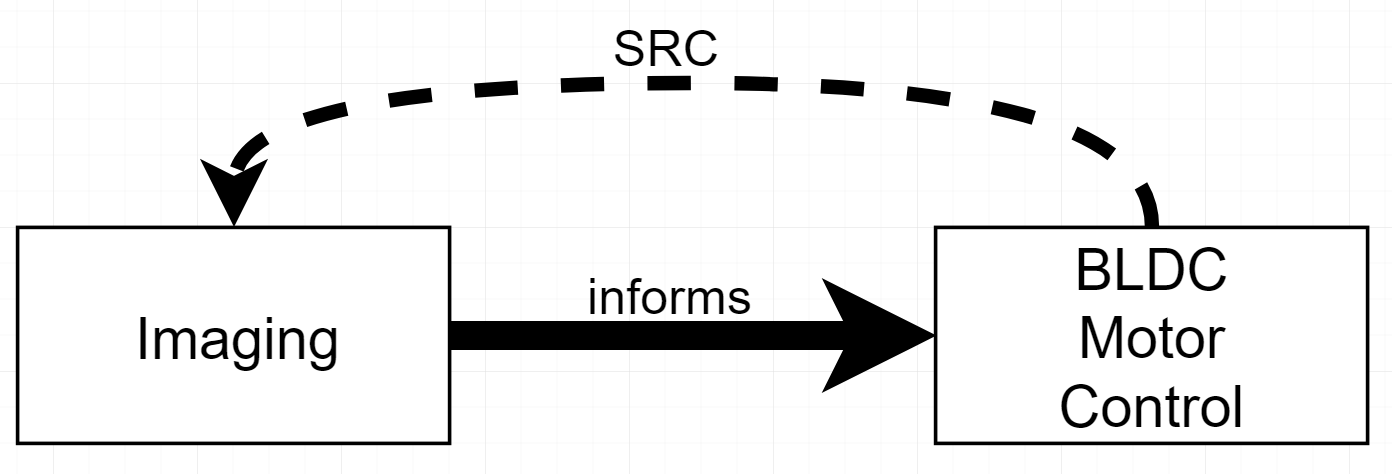
\includegraphics[width=.7\linewidth]{09_Figures/Payload-Summary-Block-Diagram.png}
		\caption{Payload Flow of Influence}
		\label{fig:Payload-Summary-Block-Diagram}
	\end{figure}
	\FloatBarrier
	
	The imaging system will have two cameras to increase field of view and improve reliability. Each camera will have a dedicated Image Processing Unit (IPU). For each image taken, the IPUs will determine if the target is in the frame of the image. If the target is found by one of the cameras, the location of the target in the frame and the pixel size of the target will be processed in order to determine the desired change in the angular position of the fore section. The motor control system then attempts to reach that setpoint. This system control flow from sensors to actuator is shown in Figure \ref{fig:payloadWOO}.
	
	\bigbreak
	
	The multiple processing systems on board will allow for concurrency in computation and real-time target tracking and mechanical response. ``Real-time" computing systems guarantee a correct system response within a specified time constraint. For this application, a ``real-time" response is defined by the window of the flight experiment. This payload's image processing system has hard real-time requirements because of the short experimental window in which SRC actuation must center targets in the field of view of one of its cameras.
	
	\bigbreak
	
	The entire payload will operate in a continuous loop for the duration of the experimental window.
	
	\bigbreak
	
	%payloadWOO figure blows their minds! Oh God! Its so bloody!
	\FloatBarrier
	\begin{figure}[!h]
		\centering
		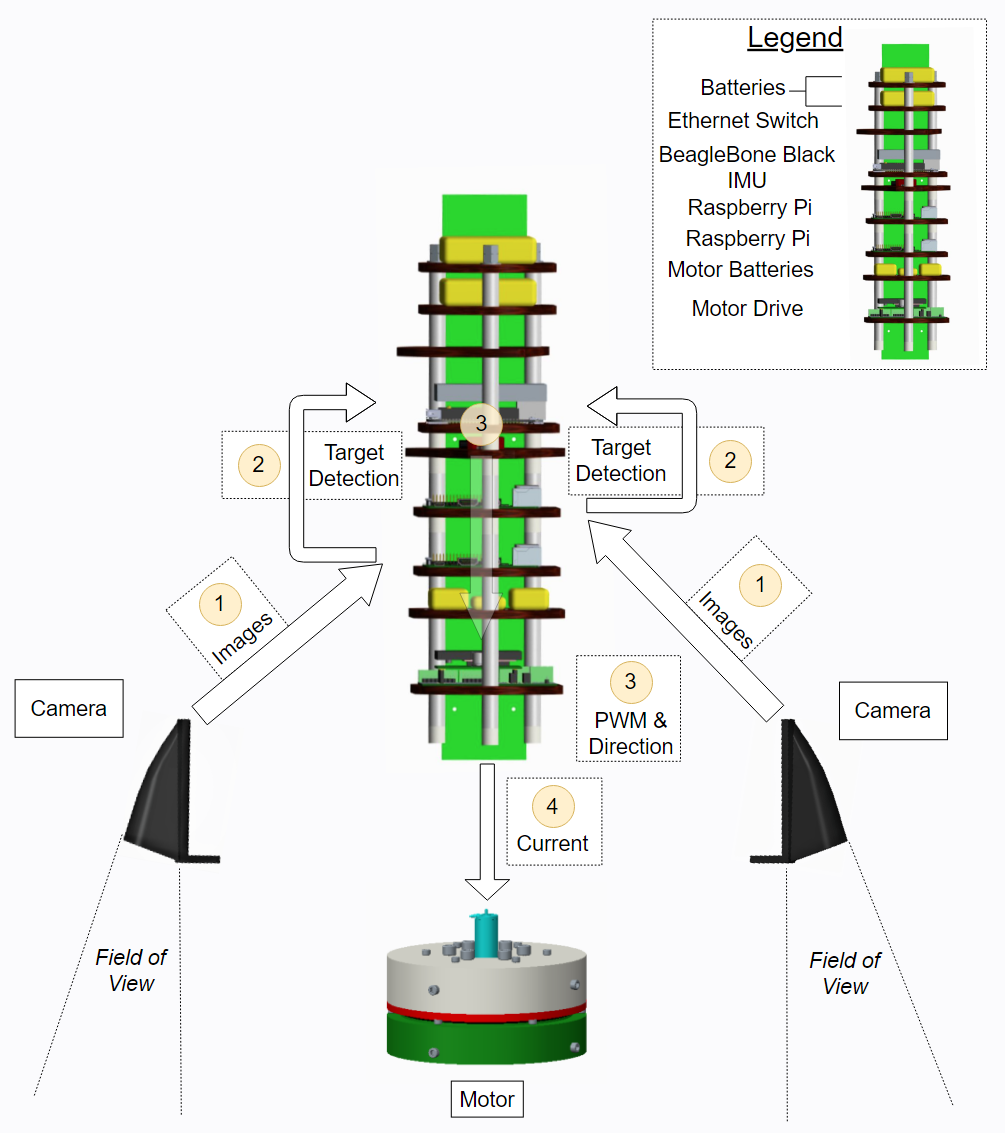
\includegraphics[width=0.85\linewidth]{09_Figures/Payload/payloadWOO.png}
		\caption{Exploded View of Payload with Dataflow Overlay}
		\label{fig:payloadWOO}
	\end{figure}
	\FloatBarrier
	
\end{document}
